\documentclass{article}
\usepackage[T1]{fontenc}
\usepackage{lmodern}
\usepackage{graphicx}
\usepackage{amsmath,amssymb}
\usepackage[a4paper,margin=2cm]{geometry}
\usepackage[absolute,overlay]{textpos}
\setlength{\TPHorizModule}{1mm}
\setlength{\TPVertModule}{1mm}
\usepackage[indonesian]{babel}
\usepackage{hyperref}
\setlength{\emergencystretch}{2em}
% unit: Halaman 39

\begin{document}

% === Halaman 39 (llm) ===

\begin{itemize}
    \item Dengan karakteristik seperti terebut, maka distribusi kemunculan huruf di dalam cipherteks relatif mendekati seragam (\textit{uniform}) dan histogramnya cenderung \textit{flat} (datar)
    \item Histogram yang flat akan menyulitkan kriptanalisis memecahkan cipherteks dengan metode analisis frekuensi
\end{itemize}

\vspace{20mm}

% deskripsi: Perbandingan antara histogram yang flat (datar) dan histogram yang bukan flat, menunjukkan distribusi frekuensi huruf A sampai Z.
% bbox normalisasi: [0.1100, 0.4500, 0.8600, 0.9100]
\begin{textblock*}{157.50mm}(23.10mm,133.65mm)
\noindent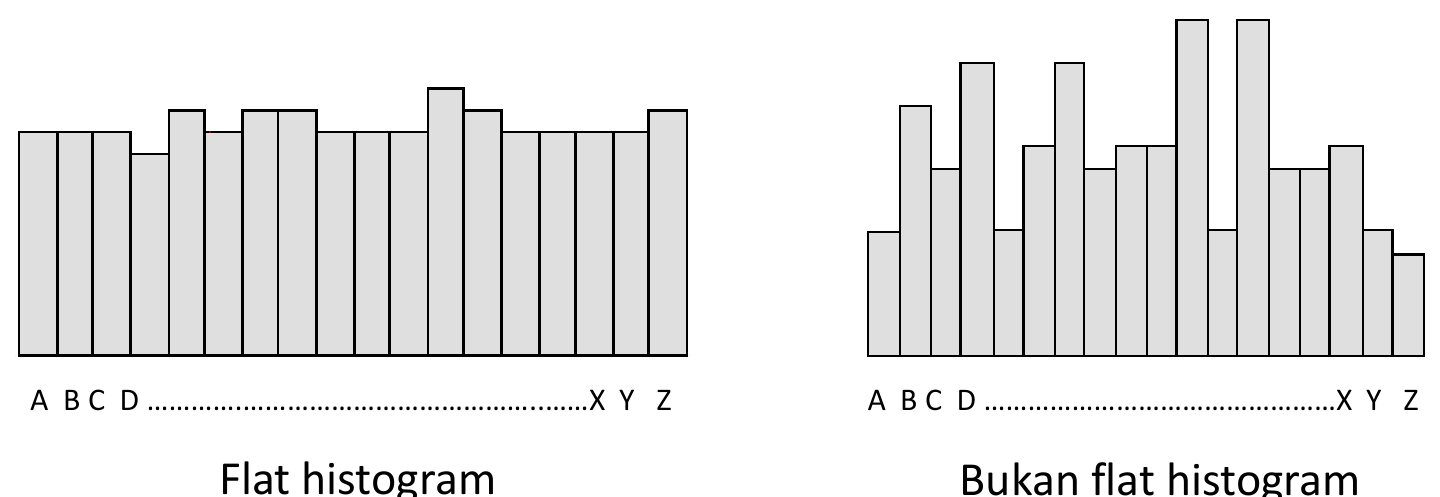
\includegraphics[width=157.50mm,height=136.62mm]{../../images/llm/page_039_img_01.png}%
\end{textblock*}

\end{document}
